\chapter{Spectral BRDF Measurement of road samples}



The design and operation of a transport system require careful consideration of numerous things, such as the installation of public lighting, minimizing light pollution, temperature control, and ensuring the visibility of road markings.
Central to addressing these considerations is to know the reflectance of the road surface, which necessitates simulations or measurements.
However, conducting these simulations or measurements is often costly due to the time requirements and the need for specialized equipment.
A key question arises: Can the reflectance of a road surface be predicted if the formulation of the surface and the reflectance of its individual components are known?
The relationship between solar albedo and BRDF provides a pathway to answering this question.
Equations \eqref{eq_white_sky_albedo} and \eqref{eq_black_sky_albedo} illustrate how solar albedo can be derived from BRDF.
This indicates that if the BRDF model can predict the BRDF for any given direction of incidence and observation, then it can also predict the solar albedo of the surface.
Chapter~\ref{ch: brdf-models} provides several BRDF models expressed as functions of incident and viewing angles.
However, these models often require additional parameters that depend on the surface's characteristics.
For instance, the ON model requires knowledge of the diffuse albedo ($\rho$) and surface roughness ($\sigma$).
For each single-material component, we can calibrate a reflectance model by fitting it to spectral BRDF measurements and extracting the relevant parameters.
Once BRDF models are established for each individual component, they can be combined to construct a hybrid BRDF model for the multi-material pavement.
This model can then be fitted to the BRDF measurements to determine the weighting factors associated with each component.
Accordingly, the BRDF of this pavement can be predicted or any direction of incidence and observation.
However, achieving this lies in obtaining accurate and reliable spectral BRDF measurements, which serve as essential input to fitting process.

To support this, this chapter first introduces 4 formulations of road samples and their constituent components.
Then it provides a spectral BRDF measurement method using the equipments developed by Cerema to measure their BRDF.
This approach is validated first through comparison with results obtained from Université Gustave Eiffel (UGE), and then through BRDF measurements on Spectralon (a material with well-known Lambertian reflection model and a given diffuse albedo).
The measured spectral BRDF results for both the composite (mix-material) and individual (single-material) samples are presented and analyzed in the last section.


%%%%%%%%%%%%%%%%%%%%%%%%%%%%%%%%%%%%%%%%%%%%%%%%%%%%%%%%%%%%%%%%%%%%%%%%%%%%%%%%%%%%%%%%%%%%%%%%%%%%%%%%%%%%%%%%%%%%
\section{Road samples}

This section first presents 4 different formulations of road samples, along with their individual constituent materials, as provided by a French company.
In order to ensure reliable BRDF measurements for each single-component sample, it is required that the surface to be measured must be flat.
For this purpose, this section then describes how to construct such samples.


%%%%%%%%%%%%%%%%%%%%%%%%%%%%%%%%%%%%%%%%%%%%%%
\subsection{4 Formulations}

The 4 formulations of road samples (F1, F2, F3, and F4) and their respective components are illustrated in Figure~\ref{fig:all-roads}, with their component proportions summarized in Table~\ref{tab:4-formulations}.
Each formulation incorporates limestone filler, a very fine powder present in small proportions. 
As such, the impact of limestone filler has been disregarded in the analysis.
Formulations F1 and F4 share similar component structures, as do F2 and F3.
The primary distinction between F1 and F4 lies in the aggregate composition: F1 incorporates a single type of rock, whereas F4 includes a mixture of two different rock types.
Meanwhile, the difference between F2 and F3 is in the binder: F2 uses bitumen, while F3 employs a pigmented synthetic binder $TiO_2$.
Across all single-component samples, the materials can be broadly classified into two categories: binders and aggregates.
The binders include bitumen and the synthetic binder.
The aggregates comprise four main types:
\begin{itemize}
    \item Garonne rock in three size fractions (0/2 mm, 2/6 mm, and 6/10 mm),
    \item Sorèze limestone (0/2 mm),
    \item Lazard rock in two size fractions (2/6 mm and 6/10 mm),
    \item Gouraudière rock (6/10 mm).
\end{itemize}


\begin{figure}[!tb]
    \centering
    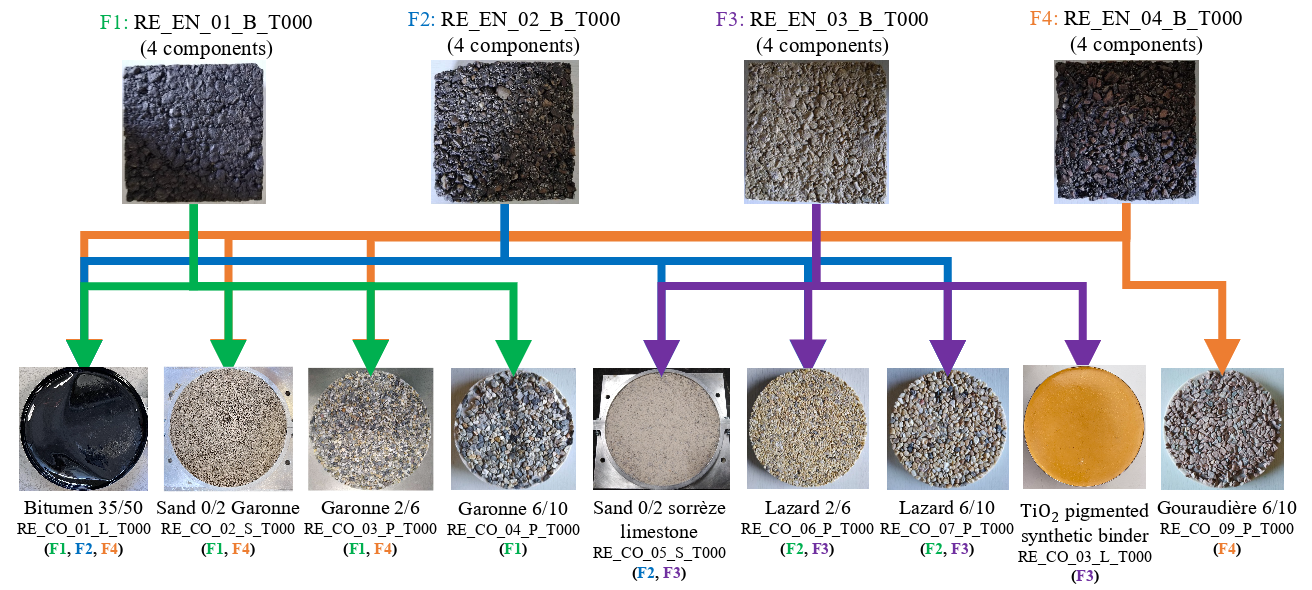
\includegraphics[width=1\linewidth]{./figures/spectral-brdf-measurements/all-roads.png}
    \caption{4 formulations of roads and their components}
    \label{fig:all-roads}
\end{figure}


\begin{table}[h]
    \centering
    \caption{4 formulations}
    \label{tab:4-formulations}
    \begin{tabular}{lcccc}
        \hline
        \hline
                               & F1       & F2       & F3       & F4       \\
        \hline
        Limestone filler       & $1.4\%$  & $2.2\%$  & $1.4\%$  & $1.9\%$  \\
        \hline
        $TiO_2$                & /        & /        & $0.5\%$  & /        \\
        \hline
        Bitumen                & $5.2\%$  & $5.3\%$  & /        & $5.4\%$  \\
        \hline
        Synthetic binder       & /        & /        & $5.4\%$  & /        \\
        \hline
        Garonne (0/2)          & $31.1\%$ & /        & /        & $29.5\%$ \\
        \hline
        Garonne (2/6)          & $19.2\%$ & /        & /        & $19.8\%$ \\
        \hline
        Garonne (6/10)         & $43.1\%$ & /        & /        & /        \\
        \hline
        Sorèze limestone (0/2) & /        & $28.3\%$ & $27.5\%$ & /        \\
        \hline
        Lazard (2/6)           & /        & $19.5\%$ & $21\%$   & /        \\
        \hline
        Lazard (6/10)          & /        & $44.7\%$ & $44.2\%$ & /        \\
        \hline
        Gouraudière (6/10)     & /        & /        & /        & $43.4\%$ \\
        \hline
        Total                  & $100\%$  & $100\%$  & $100\%$  & $100\%$  \\
        \hline
        \hline
    \end{tabular}
\end{table}

%%%%%%%%%%%%%%%%%%%%%%%%%%%%%%%%%%%%%%%%%%%%%%
\subsection{Construction of single-material samples}

The procedure for fabricating a one-component sample with a flat surface is as follows:
\begin{enumerate}
    \item Prepare all the materials and tools including:
    \begin{itemize}
        \item 3 liquid products (as illuminated in Fig~\ref{fig:3-materials}): Renlease QZ511, REN HY956 from RenShape and Resin - RENLAM MS-1
        \item Aluminum mould, as seen in Fig~\ref{fig:mould-empty}
        \item Brush
        \item Stainless steel spatula
        \item Mixing container
        \item Clean aggregates
        \item Fontainebleau sands
    \end{itemize}

    \item Clean the mould, then install the aluminum mould and secure it with 2 screws.
    \item Coating the mould with unmold liquid Renlease QZ511 using the brush, as seen in Fig~\ref{fig:module-oil}.
    \item Put a single layer of aggregates, making sure they are as close together as possible, as seen in Fig~\ref{fig:mould-rock}.
    \item Place a layer of sand on top of the aggregate to prevent the resin from passing through the pores between the aggregates, as shown in Fig~\ref{fig:module-rock-sand}.
    \item Put $300g$ of RENLAM MS-1 resin and $100g$ of REN HY956 hardener in the mixing container, and mix them together, then put in $800g$ of Fontainebleau sand, as seen in Fig~\ref{fig:mix-3-material}.
    \item Mix the sands with the liquids in the container until homogenous, then leave them (see Fig~\ref{fig:mix-3-material-after}) for about 1 hour to warm up.
    \item Pour the homogenous glue into the mould until it is full, then make sure the top surface is flat and leave to rest for 8 hours, as seen in Fig~\ref{fig:mould-3-material}
    \item Unmould this mould and remove the sand from the surface of the aggregates, as shown in Fig~\ref{fig:sample-final}.
\end{enumerate}



\begin{figure}[!tb]
    \centering
    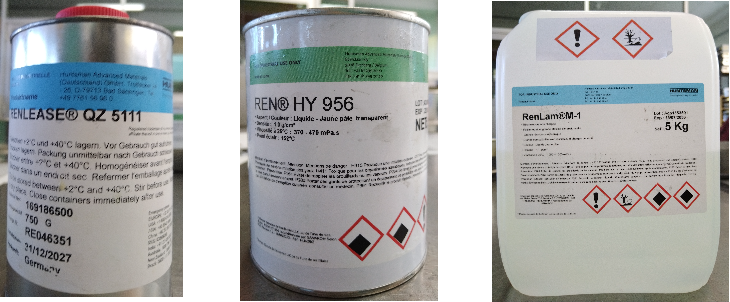
\includegraphics[width=0.9\linewidth]{./figures/spectral-brdf-measurements/3-materials.png}
    \caption{3 liquid products: Unmould liquid - Renlease QZ511 (left), Hardener - REN HY956 from RenShape (middle), Resin - RENLAM MS-1 (right)}
    \label{fig:3-materials}
\end{figure}


\begin{figure}[!tb]
    \centering
    \subfigure[Clean aluminum mould]{
        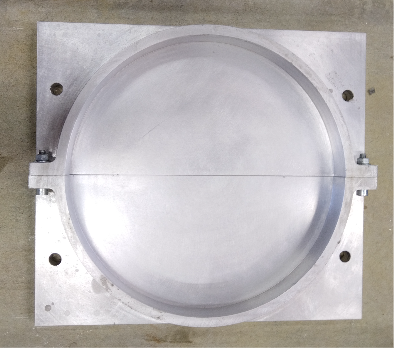
\includegraphics[width=0.45\linewidth]{./figures/spectral-brdf-measurements/module-empty.png}
        \label{fig:mould-empty}
    }
    \hfil
    \subfigure[Coating aluminum mould]{
        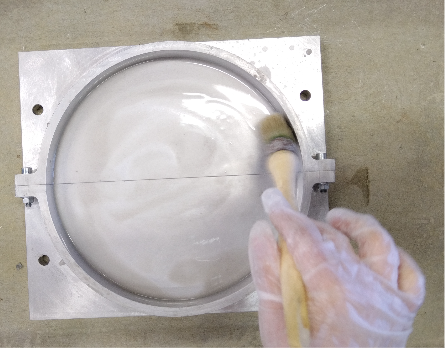
\includegraphics[width=0.45\linewidth]{./figures/spectral-brdf-measurements/module-oil.png}
        \label{fig:module-oil}
    }
    \caption{Aluminum mould}
    \label{fig:module}
\end{figure}


\begin{figure}[!tb]
    \centering
    \subfigure[Put a single layar of aggregates on the mould]{
        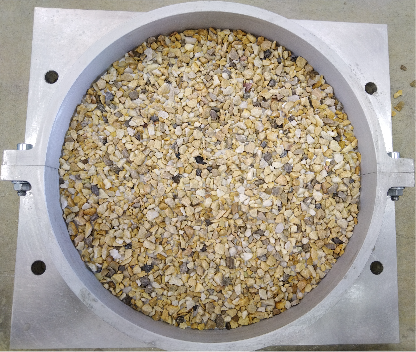
\includegraphics[width=0.45\linewidth]{./figures/spectral-brdf-measurements/module-rock.png}
        \label{fig:mould-rock}
    }
    \hfil
    \subfigure[Put a single layar of sands on the aggregates]{
        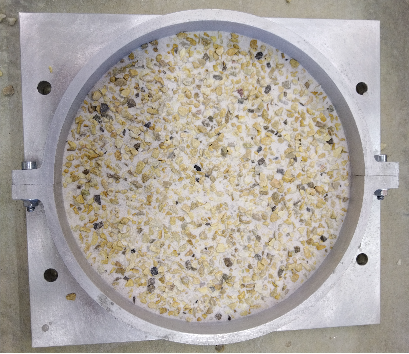
\includegraphics[width=0.45\linewidth]{./figures/spectral-brdf-measurements/module-rock-sand.png}
        \label{fig:module-rock-sand}
    }
    \caption{Placing the aggregates on the mould}
    \label{fig:aggregates}
\end{figure}


\begin{figure}[!tb]
    \centering
    \subfigure[Put all materials in the container]{
        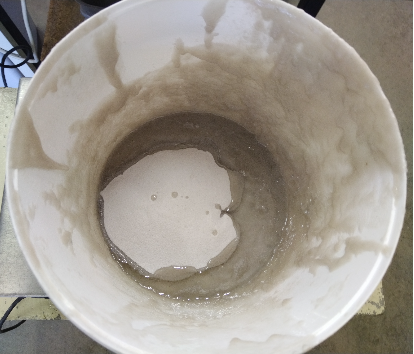
\includegraphics[width=0.45\linewidth]{./figures/spectral-brdf-measurements/mix-3-material.png}
        \label{fig:mix-3-material}
    }
    \hfil
    \subfigure[Homogenous glue after mixing]{
        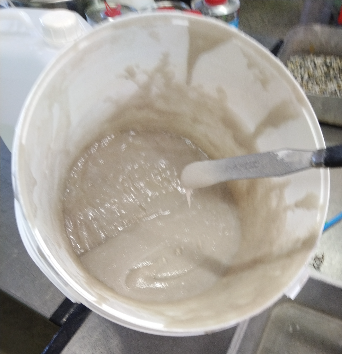
\includegraphics[width=0.45\linewidth]{./figures/spectral-brdf-measurements/mix-3-material-after.png}
        \label{fig:mix-3-material-after}
    }
    \caption{Making the glue}
    \label{fig:making-the-glue}
\end{figure}



\begin{figure}[!tb]
    \centering
    \subfigure[Pour the glue on the mould]{
        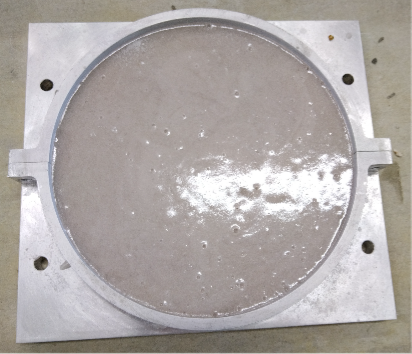
\includegraphics[width=0.45\linewidth]{./figures/spectral-brdf-measurements/module-3-materials.png}
        \label{fig:mould-3-material}
    }
    \hfil
    \subfigure[Final sample]{
        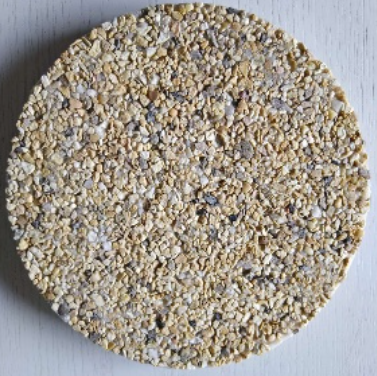
\includegraphics[width=0.45\linewidth]{./figures/spectral-brdf-measurements/sample-final.png}
        \label{fig:sample-final}
    }
    \caption{Unmold}
    \label{fig:unmould}
\end{figure}

%%%%%%%%%%%%%%%%%%%%%%%%%%%%%%%%%%%%%%%%%%%%%%%%%%%%%%%%%%%%%%%%%%%%%%%%%%%%%%%%%%%%%%%%%%%%%%%%%%%%%%%%%%%%%%%%%%%%
\section{Spectral BRDF Measurement}

This section describes a measurement set-up developed by Cerema (see in Fig.~\ref{fig:gonio}), allowing for the elimination of environmental interferences and ensuring precise control over experimental conditions.

\begin{figure}[!tb]
    \centering
    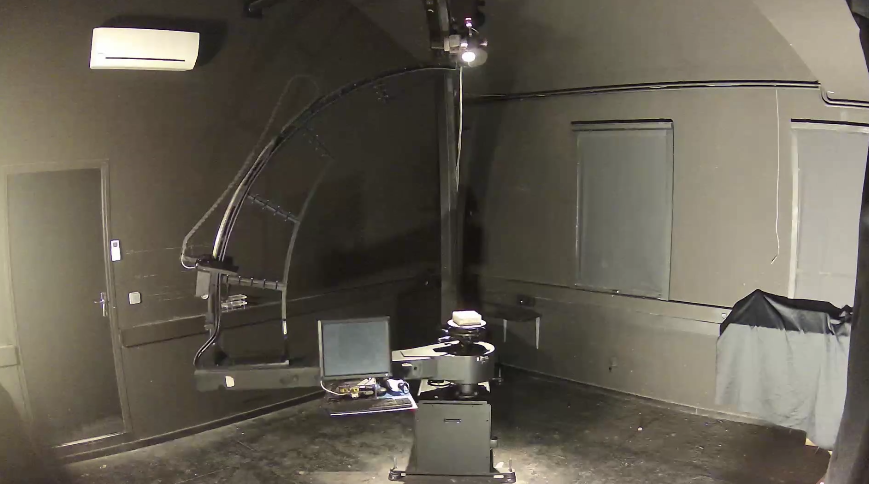
\includegraphics[width=0.9\linewidth]{./figures/optical-properties-of-road-surface/gonio-new.png}
    \caption{Gonioreflectometer (Cerema)}
    \label{fig:gonio}
\end{figure}

%%%%%%%%%%%%%%%%%%%%%%%%%%%%%%%%%%%%%%%%%%%%%%
\subsection{Spectral BRDF Measurement set-up: the Gonioreflectometer at Cerema}


The Gonioreflectometer is composed of:
\begin{itemize}
    \item light source: Halogene lamp (350nm -2500nm)
    \item reception sensor: spectroradiometer
    \item goniometer: changing the incident angle and viewing angles
\end{itemize}





\begin{figure}[!tb]
    \centering
    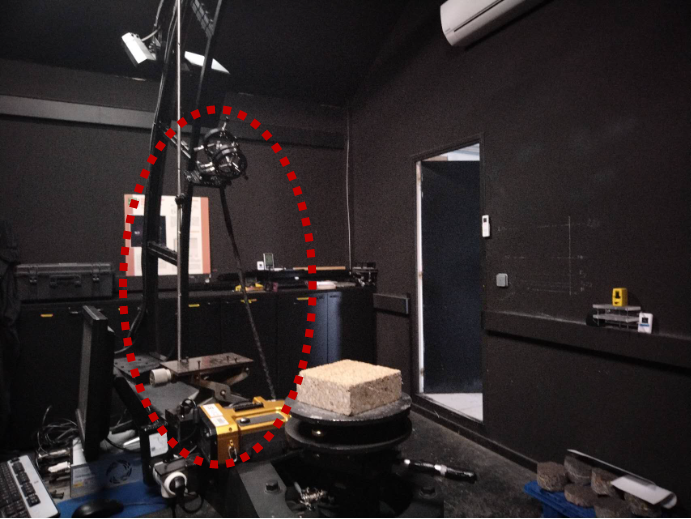
\includegraphics[width=0.9\linewidth]{./figures/spectral-brdf-measurements/gonio-spectroradiometer.png}
    \caption{Gonio-spectroradiometer (Cerema)}
    \label{fig:gonio-spectroradiometer}
\end{figure}

\begin{figure}[!tb]
    \centering
    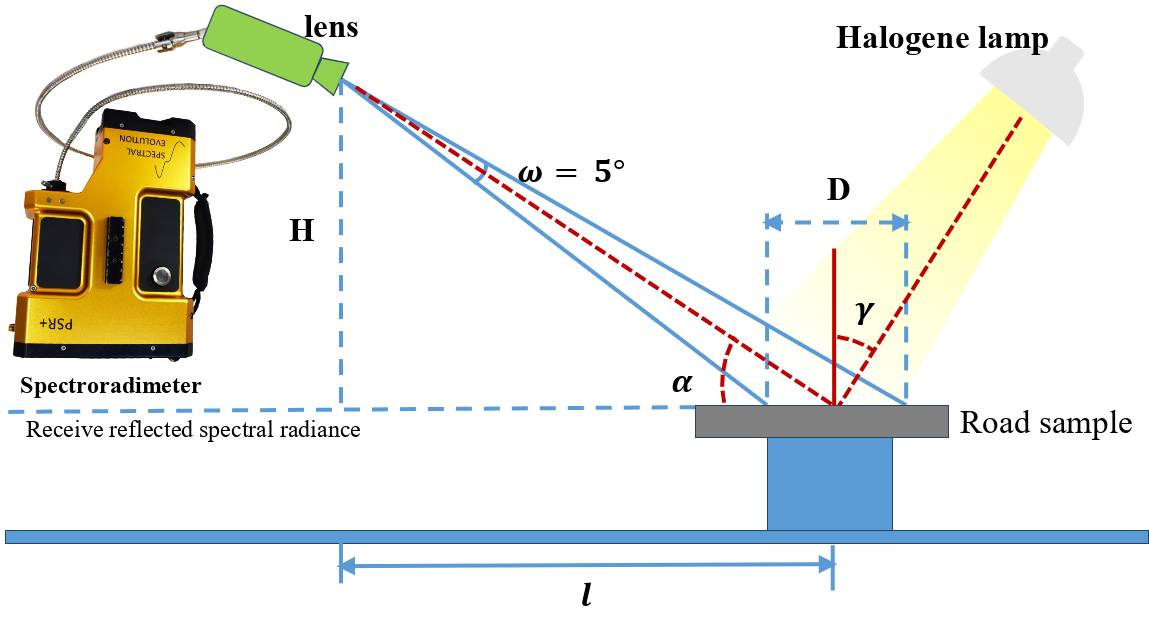
\includegraphics[width=0.9\linewidth]{./figures/spectral-brdf-measurements/gonio-simple.png}
    \caption{Gonio-spectroradiometer (Cerema)}
    \label{fig:gonio-simple}
\end{figure}

%%%%%%%%%%%%%%%%%%%%%%%%%%%%%%%%%%%%%%%%%%%%%%
\subsection{Measurement steps}

\begin{itemize}
    \item step 1 - installation of the spectroradiometer

          There are several spectroradiometers: $1^{\circ}$ and $5^{\circ}$

    \item step 2 - installation of the sample

    \item step 3 - launch the software (GonioPilotageDesAxes) to turn on the Halogene lamp

          When the software is on, then in this software
          \begin{enumerate}
              \item set the parameters
                    \begin{itemize}
                        \item choose COM3
                        \item choose where to save the result files
                    \end{itemize}

              \item turn on COM ESP301 (green means it is on)
              \item turn on the lamp (green means it is on)
              \item access the measured screen
              \item activate the remote control (yellow mean it is on)
          \end{enumerate}

    \item step 4 - launch python code to start the measurement
          \begin{enumerate}
              \item modify the $\alpha$, and change the saving sql file name for corresponding $\alpha$
              \item change the height of spectroradiometer
              \item launch the spectral evolution
              \item launch the python codes
              \item once the python codes is done, stop the spectral evolution
          \end{enumerate}

    \item step 6 - send sql file and measured radiance to Sebastian and receive the results in .csv file
\end{itemize}


\textcolor{red}{Measurement set-up:\\
    Provide the diagram of measurement set-up.
}


%%%%%%%%%%%%%%%%%%%%%%%%%%%%%%%%%%%%%%%%%%%%%%%%
\subsection{Comparison with UGE}
First we compared our results with that of UGE, to see if our measured matched with that of UGE.
For most configurations, there is a good match, but for some configurations, like large incident.
For these cases, there are direct light reaching the lens, leading to more radiance detected by the spectroradiometer.
To further validate our method, we measure the BRDF of Spectralon which offers Lambertian BRDF with given diffuse albedo.

%%%%%%%%%%%%%%%%%%%%%%%%%%%%%%%%%%%%%%%%%%%%%%%%
\subsection{Validation with Spectralon}

So here we will provide the BRDF along the wavelength ($350nm - 2500nm$) and its BRDF distribution which should be unit hemisphere.


%%%%%%%%%%%%%%%%%%%%%%%%%%%%%%%%%%%%%%%%%%%%%%%%%%%%%%%%%%%%%%%%%%%%%%%%%%%%%%%%%%%%%%%%%%%%%%%%%%%%%%%%%%%%%%%%%%%%
\section{Results}

\subsection{Methodology}

The wavelength $350nm$ to $2500nm$

Measurement scenario
\begin{itemize}
    \item $l$ - the horizontal distance between the sample and the spectroradiometer
    \item $H$ - the height difference between spectroradiometer and the sample
    \item $\gamma$ - the incident angle ($\gamma = \theta_i$): $0^{\circ} - 90^{\circ}$

    \item $\alpha$ - the observation angle ($\alpha = \frac{\pi}{2} - \theta_r$): $0^{\circ} - 90^{\circ}$

    \item $\beta$ - the angle between the vertical planes of illumination and observation ($\beta = \pi - (\phi_r - \phi_i)$)
    \item $\delta$ - the angle between the observation plane and the roadway (x) axis ($\delta = \phi_r - \pi$)
\end{itemize}


%%%%%%%%%%%%%%%%%%%%%%%%%%%%%%%%%%%%%%%%%%%%%%%%
\subsection{Results of 4 Mixed Road-Material Samples}

Figure : in the same figures, plot 4 curves respectively for F1, F2, F3, F4
For a given configuration ($\theta_i, \phi_i, \theta_r, \phi_r$): the BRDF along the wavelength ($350nm - 2500nm$)

Analyze Figure 1:
\begin{itemize}
    \item comparison between F1 and F4: 1 rock different
    \item comparison between F2 and F3: the binder different
\end{itemize}


Figure:
BRDF distribution: 2 subfigures respectively for F1 and F4


Figure:
BRDF distribution: 2 subfigures respectively for F1 and F4


Figure:
For given ($\theta_i, \phi_i, \theta_r$): plot 4 curves in polar system
Analyze Figure 4:
\begin{itemize}
    \item comparison between F1 and F4: 1 rock different
    \item comparison between F2 and F3: the binder different
\end{itemize}

%%%%%%%%%%%%%%%%%%%%%%%%%%%%%%%%%%%%%%%%%%%%%%%%
\subsection{Results of 3 Mastics}

Mastic 1 for F1 and F4: bitume and rock Garonne

Mastic 2  for F2: bitume and rock calcaire sorrèze

Mastic 3 for F3: Liant de synthèse pigmenté TiO2 and rock calcaire sorrèze


mastic 1 vs mastic 2: the rock different

mastic 2 vs mastic 3: the binder different


Figure: in the same figures, plot 4 curves respectively for F1, F2, F3, F4
For a given configuration ($\theta_i, \phi_i, \theta_r, \phi_r$): the BRDF along the wavelength ($350nm - 2500nm$)

Analyze Figure:
\begin{itemize}
    \item comparison between F1 and F4: 1 rock different
    \item comparison between F2 and F3: the binder different
\end{itemize}


Figure:
BRDF distribution: 2 subfigures respectively for F1 and F4


Figure:
BRDF distribution: 2 subfigures respectively for F1 and F4


Figure:
For given ($\theta_i, \phi_i, \theta_r$): plot 4 curves in polar system
Analyze Figure 4:
\begin{itemize}
    \item comparison between F1 and F4: 1 rock different
    \item comparison between F2 and F3: the binder different
\end{itemize}


%%%%%%%%%%%%%%%%%%%%%%%%%%%%%%%%%%%%%%%%%%%%%%%%
\subsection{Results of Single Road-Material Samples}

%%%%%%%%%%%%%%%%%%%%%%
\subsubsection{Lazard}

different size of lazard
\begin{itemize}
    \item Lazard 2/6
    \item Lazard 6/10
\end{itemize}

Figure: in the same figures, plot 4 curves respectively for 2 different size rocks
For a given configuration ($\theta_i, \phi_i, \theta_r, \phi_r$): the BRDF along the wavelength ($350nm - 2500nm$)

Figure:
BRDF distribution: 2 subfigures respectively for 2/6 and 6/10

Figure:
For given ($\theta_i, \phi_i, \theta_r$): plot 2 curves in polar system


%%%%%%%%%%%%%%%%%%%%%%
\subsubsection{Garonne}
different size of Garonne
\begin{itemize}
    \item Garonne 2/6
    \item Garonne 6/10
\end{itemize}

Figure: in the same figures, plot 4 curves respectively for 2 different size rocks
For a given configuration ($\theta_i, \phi_i, \theta_r, \phi_r$): the BRDF along the wavelength ($350nm - 2500nm$)

Figure:
BRDF distribution: 2 subfigures respectively for 2/6 and 6/10

Figure:
For given ($\theta_i, \phi_i, \theta_r$): plot 2 curves in polar system

%%%%%%%%%%%%%%%%%%%%%%
\subsubsection{Gouraudière}

Figure: in the same figures, plot 3 curves respectively for the same size rocks
For a given configuration ($\theta_i, \phi_i, \theta_r, \phi_r$): the BRDF along the wavelength ($350nm - 2500nm$)

Figure:
BRDF distribution: for Gouraudière
Comparing to Lazard and Garonne

Figure:
For given ($\theta_i, \phi_i, \theta_r$): plot 3 curves in polar system for the same size rocks






